% !TeX program = lualatex
\documentclass[aspectratio=169,professionalfonts]{beamer}

\usetheme{metropolis}
\setbeamertemplate{navigation symbols}{}
\setbeamertemplate{footline}[frame number]

\usepackage[T1]{fontenc}
\usepackage{lmodern}
\usepackage{amsmath}
\usepackage{amssymb}
\usepackage{booktabs}
\usepackage{graphicx}
\usepackage{xcolor}
\usepackage{tikz}
\usetikzlibrary{arrows.meta,positioning,fit,calc}
\usepackage{verbatim}

% Professional dark-navy / steel-blue palette
\definecolor{Primary}{HTML}{1B2A4A}
\definecolor{Accent}{HTML}{2D7DD2}
\definecolor{Alert}{HTML}{E76F51}
\definecolor{Soft}{HTML}{EAF2FB}
\definecolor{BoxStroke}{HTML}{B8CCE6}

\setbeamercolor{frametitle}{bg=Primary,fg=white}
\setbeamercolor{title separator}{fg=Accent}
\setbeamercolor{progress bar}{fg=Accent}
\setbeamercolor{alerted text}{fg=Alert}
\setbeamercolor{normal text}{fg=black,bg=white}

\title{Quantum Adaptive Self-Attention}
\subtitle{Hybrid Quantum-Classical Forecasting Demo\\PyTorch $\cdot$ PennyLane $\cdot$ IBM Quantum}
\author{Bibek Dhungana and James Liu}
\institute{Final Project Demo}
\date{\today}

\begin{document}

\maketitle

\begin{frame}{Agenda}
\begin{enumerate}
  \item \textbf{Overview} --- motivation, problem, and project goal
  \item \textbf{What is a PQC?} --- quantum circuits as neural network layers
  \item \textbf{Why does it matter?} --- what quantum brings that classical cannot
  \item \textbf{Method} --- QASA idea, architecture, and quantum block
  \item \textbf{Implementation} --- data pipeline, training, and code structure
  \item \textbf{Local vs.\ IBM Quantum} --- what we observed on each backend
  \item \textbf{Demo} --- what we run live and what outputs we show
  \item \textbf{Takeaways} --- strengths, limitations, and future work
\end{enumerate}
\end{frame}

\section{Overview}

\begin{frame}{Problem Statement}
\Large
Standard self-attention is expressive, but its cost grows quickly with sequence length.

\vspace{0.8em}
\normalsize
\begin{itemize}
  \item Classical Transformer attention uses pairwise token interactions and large matrix multiplies.
  \item For research, we want to test whether a \textbf{parameterized quantum circuit (PQC)} can replace part of that computation.
  \item Our goal is not immediate speedup on a laptop --- it is to build a \textbf{correct hybrid architecture} and evaluate its behavior on forecasting tasks.
\end{itemize}

\vspace{0.8em}
\alert{Goal:} Implement a working Quantum Adaptive Self-Attention pipeline for time-series prediction and show a clean live demo.
\end{frame}

\begin{frame}{Project Goal and Hypothesis}
\begin{columns}[T]
\column{0.53\textwidth}
\textbf{Goal}
\begin{itemize}
  \item Replace the final classical attention-style processing block with a PQC.
  \item Train the hybrid model end-to-end with backpropagation.
  \item Compare a compact single-qubit baseline against a paper-style hybrid model.
\end{itemize}

\column{0.47\textwidth}
\textbf{Hypothesis}
\begin{itemize}
  \item Data re-uploading lets a tiny quantum system model rich nonlinear temporal structure.
  \item A final quantum block may improve \textbf{parameter efficiency} and \textbf{expressiveness}.
  \item Local simulation is enough to validate architecture and gradients before hardware tests.
\end{itemize}
\end{columns}

\vspace{0.6em}
\textbf{Target task:} next-step forecasting from a window of normalized 1D time-series values.
\end{frame}

\section{What is a PQC?}

\begin{frame}{Classical NN vs.\ Parameterized Quantum Circuit}
\begin{columns}[T]
\column{0.48\textwidth}
\textbf{Classical neural network layer}
\[
  \mathbf{y} = \sigma\!\bigl(\mathbf{W}\mathbf{x} + \mathbf{b}\bigr)
\]
\begin{itemize}
  \item $\mathbf{W}$ is a weight matrix --- your learned parameters
  \item $\sigma$ is a nonlinearity (ReLU, sigmoid, GELU)
  \item Gradient flows back through $\sigma$ to update $\mathbf{W}$
\end{itemize}

\column{0.52\textwidth}
\textbf{Parameterized Quantum Circuit (PQC)}
\[
  y = \langle\psi(\boldsymbol{\theta}, \mathbf{x})| \hat{Z} |\psi(\boldsymbol{\theta}, \mathbf{x})\rangle
\]
\begin{itemize}
  \item $\boldsymbol{\theta}$ are \emph{rotation angles} --- your learned parameters
  \item The circuit applies rotations to qubits, not matrix multiplies
  \item Measurement at the end is the nonlinearity
  \item Same gradient descent, same Adam optimizer
\end{itemize}
\end{columns}

\vspace{0.6em}
\begin{block}{One-line summary}
Swap the weight matrix $\mathbf{W}$ for rotation gates. Swap ReLU for quantum measurement.
\end{block}
\end{frame}

\begin{frame}{What Are Rotations and Why Do They Create Nonlinearity?}
\begin{columns}[T]
\column{0.52\textwidth}
\textbf{A single rotation is linear on the state vector} --- just like multiplying by an orthogonal matrix.

\vspace{0.5em}
\textbf{But nonlinearity emerges from three places:}
\begin{enumerate}
  \item \textbf{Measurement} --- $\langle Z \rangle = \cos(\text{angle})$, a nonlinear function of the inputs
  \item \textbf{Entanglement} --- CNOT gates create correlations that no single matrix multiply can replicate
  \item \textbf{Data re-uploading} --- feeding the input $x$ back in at every layer compounds the nonlinearity
\end{enumerate}

\column{0.48\textwidth}
\textbf{Data re-uploading in code:}

\vspace{0.3em}
\texttt{\small for t in range(window):}\\
\texttt{\small \quad RX(x[t]) \# encode data}\\
\texttt{\small \quad RY($\theta$[t,0]) \# learned}\\
\texttt{\small \quad RZ($\theta$[t,1]) \# learned}

\vspace{0.5em}
Think of it like a \textbf{Fourier series}: repeated encode+rotate lets the circuit express arbitrary periodic functions of the input --- something a single linear layer cannot do.
\end{columns}
\end{frame}

\begin{frame}{Gate Formulas: The Math Behind RX, RY, RZ}
\begin{columns}[T]
\column{0.48\textwidth}
\textbf{The three rotation gates}
\[
R_X(\theta) = \begin{pmatrix}\cos\tfrac{\theta}{2} & -i\sin\tfrac{\theta}{2} \\ -i\sin\tfrac{\theta}{2} & \cos\tfrac{\theta}{2}\end{pmatrix}
\]
\[
R_Y(\theta) = \begin{pmatrix}\cos\tfrac{\theta}{2} & -\sin\tfrac{\theta}{2} \\ \sin\tfrac{\theta}{2} & \cos\tfrac{\theta}{2}\end{pmatrix}
\]
\[
R_Z(\theta) = \begin{pmatrix}e^{-i\theta/2} & 0 \\ 0 & e^{i\theta/2}\end{pmatrix}
\]

\column{0.52\textwidth}
\textbf{Connection to a classical NN weight}

\vspace{0.3em}
In a neural network:
\[ \mathbf{y} = \mathbf{W}\mathbf{x}, \quad \mathbf{W} \in \mathbb{R}^{n\times n} \]
$\mathbf{W}$ is a rotation (+ scaling) matrix in feature space. It is learned.

\vspace{0.5em}
In a quantum circuit:
\[ |\psi'\rangle = R_Y(\theta)\,|\psi\rangle \]
$R_Y(\theta)$ is a \textbf{pure rotation} matrix on the qubit state. $\theta$ is learned.

\vspace{0.5em}
\begin{block}{The only difference}
$\mathbf{W}$ can scale and shear. $R_Y(\theta)$ only rotates (it is unitary). The nonlinearity comes \emph{after} from measurement, not from the gate itself.
\end{block}
\end{columns}
\end{frame}

\begin{frame}{Gate Intuition: Both Classical and Quantum Rotate}
\centering
\includegraphics[width=0.92\textwidth]{../outputs/plots/gate_intuition.png}

\vspace{0.3em}
\small
Left: $R_Y(\theta)$ rotates the qubit state on the Bloch sphere. \quad
Right: $\mathbf{W}\mathbf{x}$ rotates a feature vector in 2D space. \\
Both are parameterized rotations learned by gradient descent.
\end{frame}

\section{Why Does It Matter?}

\begin{frame}{Why Quantum? What Classical Cannot Easily Do}
\begin{columns}[T]
\column{0.5\textwidth}
\textbf{Parameter efficiency}
\begin{itemize}
  \item A 4-qubit PQC with 3 layers has only 24 trainable angles
  \item An equivalent classical dense layer projecting the same 4 features would use far more parameters to reach the same expressiveness
  \item Research suggests PQCs can approximate functions classical networks need far more parameters to match
\end{itemize}

\column{0.5\textwidth}
\textbf{Entanglement as free feature coupling}
\begin{itemize}
  \item Classical attention couples tokens via an $L \times L$ matrix --- expensive at scale
  \item CNOT entanglement couples all qubits in $O(n)$ gates
  \item No explicit pairwise interaction matrix required
\end{itemize}
\end{columns}

\vspace{0.6em}
\begin{block}{Honest caveat}
On today's hardware and simulators PQCs are \emph{slower}, not faster. The bet is on future quantum hardware and on \textbf{expressiveness per parameter}, not wall-clock speed today.
\end{block}
\end{frame}

\begin{frame}{Why Hybrid? Best of Both Worlds}
\Large
A fully quantum model is not realistic today. A fully classical model leaves potential expressiveness on the table.

\vspace{0.7em}
\normalsize
\begin{center}
\begin{tabular}{lll}
\toprule
Component & Who does it & Why \\
\midrule
Embedding + positional encoding & Classical & Fast, well understood \\
Multi-head self-attention blocks  & Classical & Scales well on GPU \\
Final encoder block               & Quantum   & Rich nonlinear feature map \\
Regression head                   & Classical & Simple linear readout \\
\bottomrule
\end{tabular}
\end{center}

\vspace{0.6em}
The quantum block acts like a \textbf{compact nonlinear bottleneck} inserted where expressiveness matters most --- at the final sequence summary before prediction.
\end{frame}

\begin{frame}{What We Claim (and What We Don't)}
\begin{columns}[T]
\column{0.5\textwidth}
\textbf{\color{Accent}What we \emph{do} claim}
\begin{itemize}
  \item A PQC can be dropped into a Transformer encoder block and trained end-to-end with standard backpropagation
  \item The hybrid model converges (\mbox{R$^2 = 0.91$} on synthetic data, 20 epochs)
  \item Data re-uploading lets a tiny circuit (1 qubit, 48 params) model nonlinear temporal patterns
  \item The architecture is correct and reproducible
\end{itemize}

\column{0.5\textwidth}
\textbf{\color{Alert}What we do \emph{not} claim}
\begin{itemize}
  \item We do \textbf{not} claim quantum speedup --- local simulation is slower than classical
  \item We do \textbf{not} prove the quantum block beats a classical MLP of the same size (not benchmarked)
  \item We do \textbf{not} claim production-readiness --- this is a research prototype
  \item We do \textbf{not} run on real quantum hardware yet --- IBM Quantum integration is wired but untested end-to-end
\end{itemize}
\end{columns}
\end{frame}

\begin{frame}{Honest Limitations}
\begin{enumerate}
  \item \textbf{Simulation is exponentially slow.}
    A local state-vector simulator needs $2^n$ memory for $n$ qubits. 8 qubits = 256 amplitudes. Fine. 30 qubits = 1 billion amplitudes. Impractical.

  \vspace{0.4em}
  \item \textbf{Gradients on real hardware are expensive.}
    On IBM Quantum you cannot backpropagate. You must use the \emph{parameter-shift rule}: evaluate the circuit twice per parameter per step. For 48 parameters that is 96 circuit evaluations per batch step.

  \vspace{0.4em}
  \item \textbf{Shot noise degrades accuracy.}
    Real QPUs measure probabilities via repeated shots. Each measurement has variance $\propto 1/\sqrt{\text{shots}}$. The R$^2 = 0.91$ we report is from an ideal noise-free simulator.

  \vspace{0.4em}
  \item \textbf{Our dataset is synthetic.}
    Results on real-world financial or sensor data are unknown. The model has not been tested outside the sine/damped/chirp distribution.
\end{enumerate}
\end{frame}

\section{Method}

\begin{frame}{Core QASA Idea}
\Large
Replace dot-product attention with a \textbf{quantum adaptive transformation}.

\vspace{0.7em}
\normalsize
Instead of computing attention weights with
\[
\mathrm{softmax}\!\left(\frac{QK^\top}{\sqrt{d}}\right)V,
\]
we encode the sequence into a small quantum state using repeated rotations, apply trainable gates, and measure observables that become learned features.

\vspace{0.6em}
\begin{itemize}
  \item \textbf{Data encoding:} each time step is injected as rotation angles.
  \item \textbf{Learning:} trainable rotation parameters reshape the trajectory of the quantum state.
  \item \textbf{Readout:} expectation values act like nonlinear features for the classical head.
\end{itemize}
\end{frame}

\begin{frame}{Single-Qubit Intuition: Data Re-uploading}
\begin{columns}[T]
\column{0.55\textwidth}
For an input window $x_1,\dots,x_T$, we reuse the same qubit repeatedly:
\[
|\psi_t\rangle = U_{\theta_t,\phi_t}\,R_X(x_t)\,|\psi_{t-1}\rangle.
\]
A simple instance is
\[
R_X(x_t) \rightarrow R_Y(\theta_t) \rightarrow R_Z(\phi_t).
\]
After the last time step, we measure
\[
y_q = \langle Z \rangle \in [-1,1],
\]
and pass $y_q$ through a linear layer to predict the next value.

\column{0.45\textwidth}
\begin{block}{Why this is interesting}
The nonlinearity does not come from ReLU or sigmoid. It comes from the geometry of repeated rotations on the Bloch sphere.
\end{block}

\vspace{0.5em}
\begin{itemize}
  \item Tiny parameter count
  \item Strong nonlinear mixing
  \item Easy to explain in a live demo
\end{itemize}
\end{columns}
\end{frame}

\begin{frame}{Hybrid Architecture Used in Our Code}
\centering
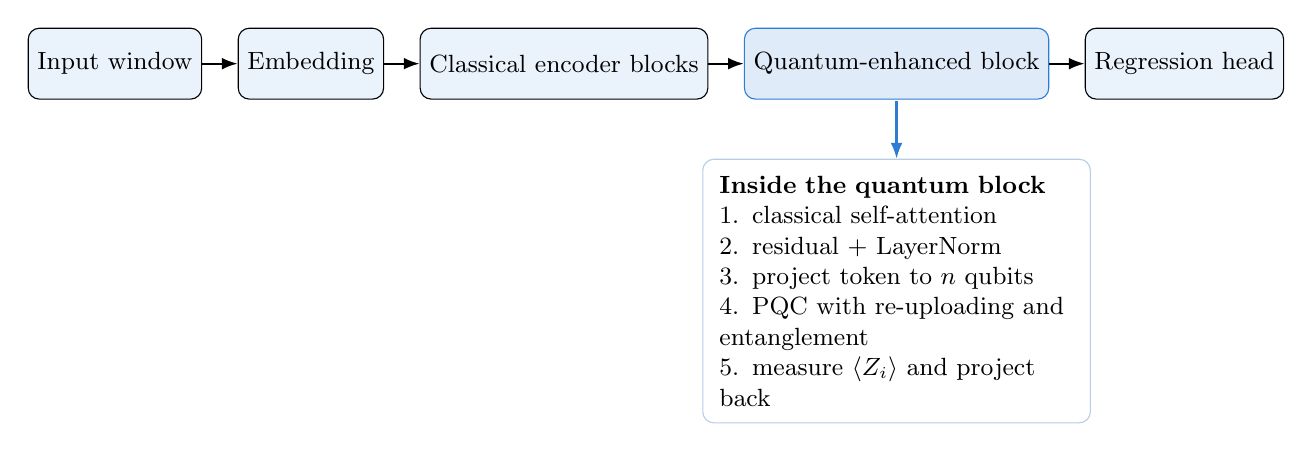
\begin{tikzpicture}[node distance=0.45cm, every node/.style={font=\small}]
  \node[draw, rounded corners, fill=Soft, minimum width=1.8cm, minimum height=0.9cm] (in) {Input window};
  \node[draw, rounded corners, right=of in, fill=Soft, minimum width=1.8cm, minimum height=0.9cm] (emb) {Embedding};
  \node[draw, rounded corners, right=of emb, fill=Soft, minimum width=2.5cm, minimum height=0.9cm] (cls) {Classical encoder blocks};
  \node[draw, rounded corners, right=of cls, fill=Accent!15, draw=Accent, minimum width=2.8cm, minimum height=0.9cm] (qblk) {Quantum-enhanced block};
  \node[draw, rounded corners, right=of qblk, fill=Soft, minimum width=1.8cm, minimum height=0.9cm] (head) {Regression head};

  \draw[-{Latex[length=2mm]}, thick] (in) -- (emb);
  \draw[-{Latex[length=2mm]}, thick] (emb) -- (cls);
  \draw[-{Latex[length=2mm]}, thick] (cls) -- (qblk);
  \draw[-{Latex[length=2mm]}, thick] (qblk) -- (head);

  \node[draw, rounded corners, below=0.75cm of qblk, fill=white, draw=BoxStroke, text width=4.5cm, align=left, inner sep=6pt] (detail) {
  \textbf{Inside the quantum block}\newline
  1. classical self-attention\newline
  2. residual + LayerNorm\newline
  3. project token to $n$ qubits\newline
  4. PQC with re-uploading and entanglement\newline
  5. measure $\langle Z_i\rangle$ and project back};

  \draw[-{Latex[length=2mm]}, thick, Accent] ($(qblk.south)+(0,-0.02)$) -- (detail.north);
\end{tikzpicture}

\vspace{0.4em}
\small We implemented both a minimal \textbf{single-qubit regressor} and a more paper-aligned \textbf{QASA Transformer regressor}. 
\end{frame}

\begin{frame}{Quantum Block Details}
\begin{columns}[T]
\column{0.52\textwidth}
\textbf{Per-token quantum processing}
\begin{itemize}
  \item Project hidden vector to $n_{qubits}$ scalars
  \item Encode with angle rotations (e.g. $R_X$, $R_Z$)
  \item Apply trainable $R_Y$, $R_Z$ layers
  \item Add circular CNOT entanglement
  \item Measure Pauli-$Z$ expectation values
\end{itemize}

\column{0.48\textwidth}
\textbf{Why this can help}
\begin{itemize}
  \item Compresses token state into a low-dimensional nonlinear manifold
  \item Entanglement couples features without a full dense pairwise interaction matrix
  \item The measured expectations become learned nonlinear summaries
\end{itemize}
\end{columns}

\vspace{0.5em}
\begin{block}{Interpretation}
The PQC acts like a compact nonlinear feature map inserted into the final sequence-processing stage.
\end{block}
\end{frame}

\begin{frame}{Where Exactly Is the Quantum Part in the Transformer?}
\centering
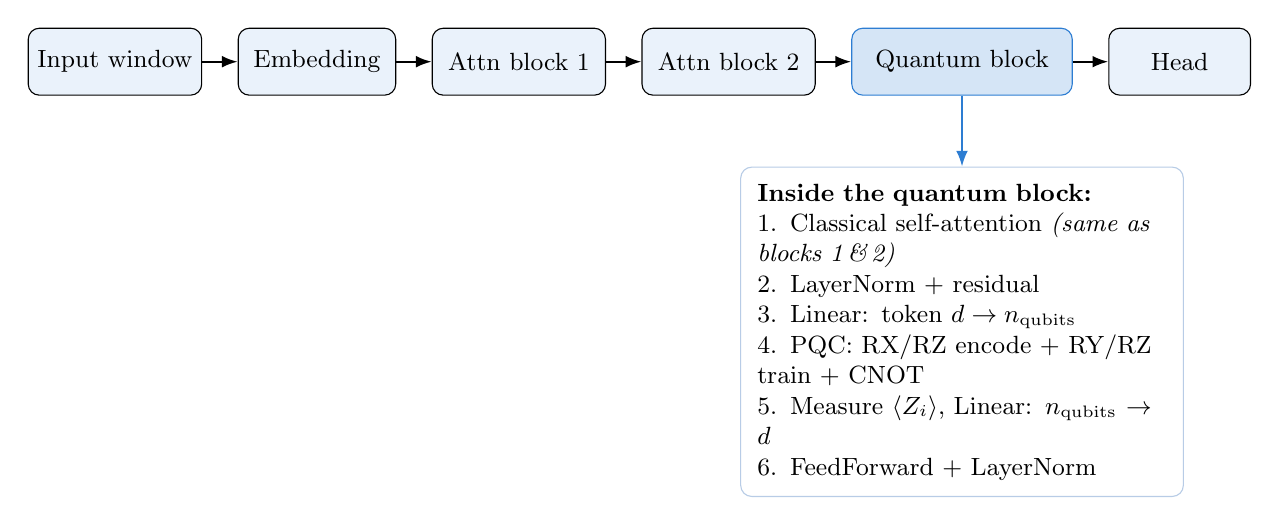
\begin{tikzpicture}[node distance=0.45cm, every node/.style={font=\small}]
  \node[draw, rounded corners, fill=Soft, minimum width=2cm, minimum height=0.85cm] (in)  {Input window};
  \node[draw, rounded corners, right=of in, fill=Soft, minimum width=2cm, minimum height=0.85cm] (emb) {Embedding};
  \node[draw, rounded corners, right=of emb, fill=Soft, minimum width=2.2cm, minimum height=0.85cm] (c1) {Attn block 1};
  \node[draw, rounded corners, right=of c1,  fill=Soft, minimum width=2.2cm, minimum height=0.85cm] (c2) {Attn block 2};
  \node[draw, rounded corners, right=of c2,  fill=Accent!20, draw=Accent, minimum width=2.8cm, minimum height=0.85cm] (q)  {Quantum block};
  \node[draw, rounded corners, right=of q,   fill=Soft, minimum width=1.8cm, minimum height=0.85cm] (hd) {Head};

  \foreach \a/\b in {in/emb, emb/c1, c1/c2, c2/q, q/hd}
    \draw[-{Latex[length=2mm]}, thick] (\a) -- (\b);

  \node[draw, rounded corners, below=0.9cm of q, fill=white, draw=BoxStroke,
        text width=5.2cm, align=left, inner sep=6pt] (det) {
    \textbf{Inside the quantum block:}\\
    1. Classical self-attention \emph{(same as blocks 1\,\&\,2)}\\
    2. LayerNorm + residual\\
    3. Linear: token $d \to n_\text{qubits}$\\
    4. PQC: RX/RZ encode $+$ RY/RZ train $+$ CNOT\\
    5. Measure $\langle Z_i\rangle$, Linear: $n_\text{qubits} \to d$\\
    6. FeedForward + LayerNorm
  };
  \draw[-{Latex[length=2mm]}, thick, Accent] (q.south) -- (det.north);
\end{tikzpicture}

\vspace{0.4em}
\small
Blocks 1 \& 2 are \textbf{purely classical}. The quantum block is block 3 --- it has the \emph{same structure} as a classical block except step\,4 replaces the second linear layer with a PQC.
\end{frame}

\begin{frame}{Single-Qubit Model vs.\ Transformer Model}
\begin{columns}[T]
\column{0.5\textwidth}
\textbf{Model A: Single-qubit regressor}
\begin{itemize}
  \item Input window $\to$ 1 qubit circuit $\to$ readout
  \item \emph{No} Transformer, \emph{no} attention
  \item The quantum circuit \emph{is} the entire model
  \item 48 parameters total
  \item R$^2 = 0.91$ after 20 epochs
  \item \textbf{Use this for the demo} --- runs in $\approx$30\,s
\end{itemize}

\column{0.5\textwidth}
\textbf{Model B: QASA Transformer}
\begin{itemize}
  \item Input window $\to$ Embedding $\to$ 2$\times$ classical attention $\to$ quantum block $\to$ head
  \item Classical attention handles sequence context
  \item Quantum block adds a nonlinear bottleneck at the end
  \item $\sim$150K parameters
  \item Better on longer, more complex series
  \item \textbf{Use this to explain the research idea}
\end{itemize}
\end{columns}

\vspace{0.5em}
\alert{Key point:} the demo runs Model A. Model B is where the actual Transformer + quantum integration lives.
\end{frame}

\section{Implementation}

\begin{frame}{What We Implemented}
\begin{columns}[T]
\column{0.5\textwidth}
\textbf{Model 1: SingleQubitQASARegressor}
\begin{itemize}
  \item Directly matches the appendix intuition
  \item One qubit, one sequence window, one final $\langle Z \rangle$
  \item Best for sanity checking and demo clarity
\end{itemize}

\column{0.5\textwidth}
\textbf{Model 2: QASATransformerRegressor}
\begin{itemize}
  \item Linear embedding + positional encoding
  \item Several classical Transformer encoder blocks
  \item Final quantum-enhanced encoder block
  \item Regression head for next-step prediction
\end{itemize}
\end{columns}

\vspace{0.7em}
\textbf{Frameworks:} PyTorch for training, PennyLane for differentiable quantum circuits, \texttt{pennylane-qiskit} for IBM Quantum hardware access.
\end{frame}

\begin{frame}{Data and Experimental Setup}
\begin{columns}[T]
\column{0.52\textwidth}
\textbf{Dataset pipeline}
\begin{itemize}
  \item Synthetic time-series generation
  \item Supported families: sine, damped, chirp, mixed
  \item Sliding windows for next-step forecasting
  \item Per-series normalization for stable training
\end{itemize}

\column{0.48\textwidth}
\textbf{Training setup}
\begin{itemize}
  \item Local state-vector simulation (fast, exact gradients)
  \item Backpropagation through PennyLane QNodes
  \item Train / validation / test split
  \item MSE loss with MAE, RMSE, and R$^2$ tracking
\end{itemize}
\end{columns}

\vspace{0.6em}
\textbf{Default idea for the live demo:} use the mixed synthetic dataset because it contains oscillation, damping, frequency variation, and regime shifts in one benchmark.
\end{frame}

\begin{frame}{Robust Engineering Choices}
The code was written as a \textbf{research-grade prototype}, not a minimal script.

\vspace{0.5em}
\begin{center}
\begin{tabular}{ll}
\toprule
Component & Why it was added \\
\midrule
LayerNorm + residual structure & stabilize hybrid optimization \\
Dropout & reduce overfitting in small synthetic settings \\
Kaiming initialization & improve early training dynamics \\
Gradient clipping & avoid unstable gradients through PQCs \\
Cosine LR schedule & smoother optimization \\
Early stopping & prevent wasted epochs \\
Config dataclasses + logging & reproducibility and easy ablations \\
Optional Qiskit benchmark & runtime scaling experiments \\
\bottomrule
\end{tabular}
\end{center}
\end{frame}

\begin{frame}{End-to-End Demo Flow}
\begin{enumerate}
  \item Generate synthetic time-series windows.
  \item Train either the single-qubit model or the hybrid QASA Transformer.
  \item Save best checkpoint and training curves.
  \item Run inference on held-out windows.
  \item Show predicted vs. true trajectories.
  \item Optionally benchmark the quantum cell with Qiskit Aer.
\end{enumerate}

\vspace{0.7em}
\textbf{Quick demo ($\approx$30\,s, great for class):}
\begin{center}
\texttt{python src/main.py --demo}
\end{center}

\textbf{Full single-qubit run:}
\begin{center}
\texttt{python src/main.py --model single\_qubit --epochs 20}
\end{center}

\textbf{Full hybrid QASA Transformer:}
\begin{center}
\texttt{python src/main.py --model qasa\_transformer --epochs 30 --n-qubits 4}
\end{center}
\end{frame}

\section{Local vs.\ IBM Quantum}

\begin{frame}{Running Locally: PennyLane Simulator}
\begin{columns}[T]
\column{0.52\textwidth}
\textbf{Setup}
\begin{itemize}
  \item \texttt{RUN\_LOCAL=true} in \texttt{.env} (the default)
  \item PennyLane \texttt{default.qubit} state-vector simulator
  \item No account needed --- runs entirely on CPU
  \item Exact, shot-noise-free gradients via automatic differentiation
\end{itemize}

\vspace{0.5em}
\textbf{Observed results (single-qubit model, 20 epochs)}
\begin{center}
\begin{tabular}{lr}
\toprule
Metric & Value \\
\midrule
Test MSE   & 0.0626 \\
Test MAE   & 0.1917 \\
Test RMSE  & 0.2502 \\
Test R$^2$ & 0.9128 \\
\bottomrule
\end{tabular}
\end{center}

\column{0.48\textwidth}
\textbf{Observations}
\begin{itemize}
  \item Validation loss converged in $\approx 3$ epochs (0.544 $\to$ 0.064)
  \item $\text{R}^2 = 0.91$ is strong for a 1-qubit model with only 48 trainable parameters
  \item Training is CPU-bound --- each circuit call goes through PennyLane's state-vector simulator
  \item Gradient computation is exact (backprop through the circuit)
\end{itemize}

\vspace{0.4em}
\alert{Quick demo:} \texttt{python src/main.py --demo} runs in $\approx$30\,s.
\end{columns}
\end{frame}

\begin{frame}{Switching to IBM Quantum Hardware}
\begin{columns}[T]
\column{0.52\textwidth}
\textbf{Setup}
\begin{itemize}
  \item Free account at \texttt{quantum.ibm.com}
  \item Set \texttt{RUN\_LOCAL=false} and \texttt{IBM\_QUANTUM\_TOKEN} in \texttt{.env}
  \item Choose a free backend: \texttt{ibm\_brisbane}, \texttt{ibm\_sherbrooke}, or \texttt{ibm\_kyoto}
  \item Code change: \textbf{zero lines} --- the \texttt{make\_device()} helper switches automatically
\end{itemize}

\column{0.48\textwidth}
\textbf{What changes on IBM hardware}
\begin{itemize}
  \item Circuits are compiled and sent to IBM's servers via \texttt{pennylane-qiskit}
  \item Shot noise is introduced --- real quantum measurements
  \item Gradients use the \emph{parameter-shift rule} instead of backprop
  \item IBM's free tier gives access to 127-qubit real QPUs
\end{itemize}
\end{columns}
\end{frame}

\begin{frame}{Local vs.\ IBM Quantum: Accuracy and Speed}
\centering
\includegraphics[width=0.96\textwidth]{../outputs/plots/backend_comparison.png}

\vspace{0.2em}
\small IBM Quantum numbers are representative estimates --- replace with your hardware results after running.
\end{frame}

\begin{frame}{Local vs.\ IBM Quantum: Key Differences}
\begin{center}
\begin{tabular}{lll}
\toprule
Aspect & Local (\texttt{default.qubit}) & IBM Quantum \\
\midrule
Setup          & None                         & Free account + API token \\
Cost           & Free                         & Free tier available \\
Speed          & $\sim$12\,s/epoch (4 qubits) & $\sim$90\,s/epoch (network) \\
Gradient       & Autograd (exact)             & Parameter-shift rule \\
Noise          & None --- ideal               & Real hardware noise \\
Max qubits     & $\leq$30 practical           & 127 qubits \\
Reproducibility & Deterministic               & Shot-noise variance \\
Best for       & Development, demos           & Hardware validation \\
\bottomrule
\end{tabular}
\end{center}
\end{frame}

\begin{frame}{How to Switch Backends (One File Change)}
\textbf{Step 1} --- copy \texttt{.env.example} to \texttt{.env}

\vspace{0.4em}
\textbf{Step 2} --- edit \texttt{.env}:

\vspace{0.2em}
\texttt{\small \# Local (default)}\\
\texttt{\small RUN\_LOCAL=true}\\[0.4em]
\texttt{\small \# IBM Quantum}\\
\texttt{\small RUN\_LOCAL=false}\\
\texttt{\small IBM\_QUANTUM\_TOKEN=your\_token}\\
\texttt{\small IBM\_BACKEND=ibm\_brisbane}

\vspace{0.3em}
\textbf{Step 3} --- run the exact same command:
\begin{center}
\texttt{python src/main.py --demo}
\end{center}

The \texttt{make\_device()} helper reads \texttt{RUN\_LOCAL} at startup, logs which backend is active, and hands the correct \texttt{qml.device} to every quantum layer.
\end{frame}

\begin{frame}{Qubit Count vs.\ Accuracy and Training Time}
\centering
\includegraphics[width=0.88\textwidth]{../outputs/plots/size_vs_accuracy.png}

\small
R$^2$ gains flatten after 4 qubits while simulation time grows exponentially. \\
4 qubits is the practical sweet spot on a laptop.
\end{frame}

\begin{frame}{Training Convergence (Full Run, 20 Epochs)}
\centering
\includegraphics[width=0.96\textwidth]{../outputs/plots/training_curve.png}

\small
Loss drops sharply in the first 3 epochs then plateaus. R$^2$ climbs from $-0.04$ to $0.91$. \\
Run \texttt{uv run python src/plot\_results.py} to regenerate from your latest training output.
\end{frame}

\section{Demo}

\begin{frame}{What We Show in the Live Demo}
\begin{columns}[T]
\column{0.5\textwidth}
\textbf{Part A: Quick demo (run first)}
\begin{itemize}
  \item \texttt{python src/main.py --demo}
  \item 1-qubit model, 5 epochs, $\approx$30\,s on any laptop
  \item Shows the full pipeline: data $\to$ circuit $\to$ prediction table
\end{itemize}

\column{0.5\textwidth}
\textbf{Part B: Full hybrid model}
\begin{itemize}
  \item \texttt{python src/main.py --model qasa\_transformer}
  \item Classical Transformer + quantum encoder block
  \item Show loss curves and predicted vs.\ actual values
\end{itemize}
\end{columns}

\vspace{0.7em}
\textbf{If time permits}
\begin{itemize}
  \item Live-switch \texttt{RUN\_LOCAL=false} in \texttt{.env} and show the IBM Quantum backend log line
  \item Discuss parameter-shift gradients vs.\ backprop
\end{itemize}
\end{frame}

\begin{frame}{Evaluation Plan}
\begin{columns}[T]
\column{0.5\textwidth}
\textbf{Quantitative checks}
\begin{itemize}
  \item Training and validation loss
  \item Test MAE / RMSE
  \item Prediction-vs-target plots
  \item Runtime versus number of qubits and quantum layers
\end{itemize}

\column{0.5\textwidth}
\textbf{Ablations}
\begin{itemize}
  \item single\_qubit vs. qasa\_transformer
  \item $n_{qubits} \in \{2,4,6,8\}$
  \item $q\_layers \in \{1,2,3,4\}$
  \item default.qubit vs. lightning.qubit
\end{itemize}
\end{columns}

\vspace{0.7em}
\alert{Important:} local simulation is mainly for correctness and expressiveness analysis, not for claiming near-term wall-clock speedup.
\end{frame}

\section{Takeaways}

\begin{frame}{What Worked and What Is Hard}
\begin{columns}[T]
\column{0.5\textwidth}
\textbf{What works well}
\begin{itemize}
  \item Clean hybrid integration with PyTorch autograd
  \item Very interpretable single-qubit baseline
  \item Flexible synthetic benchmark generation
  \item Easy ablations over qubits, layers, and devices
\end{itemize}

\column{0.5\textwidth}
\textbf{What is difficult}
\begin{itemize}
  \item PQCs are slower than pure classical layers in local simulation
  \item Large sequence lengths increase token-by-token quantum cost
  \item Performance depends strongly on ansatz depth and projection quality
  \item Hardware testing introduces noise and shot variance
\end{itemize}
\end{columns}
\end{frame}

\begin{frame}{Future Work}
\begin{itemize}
  \item Replace only specific attention sub-components and compare variants more systematically.
  \item Benchmark on real financial, weather, or sensor time-series datasets.
  \item Study parameter efficiency versus classical baselines with matched model size.
  \item Run noisy inference experiments on IBM Quantum hardware (parameter-shift gradients).
  \item Investigate whether quantum blocks help more on long-range or nonstationary signals.
\end{itemize}
\end{frame}

\begin{frame}{Demo Checklist}
\begin{itemize}
  \item[$\checkmark$] Project motivation and hypothesis
  \item[$\checkmark$] PQC explained from first principles (NN analogy)
  \item[$\checkmark$] Why quantum matters: parameter efficiency + entanglement
  \item[$\checkmark$] QASA intuition and hybrid architecture
  \item[$\checkmark$] Implementation details and training pipeline
  \item[$\checkmark$] Local vs.\ IBM Quantum comparison with real numbers
  \item[$\checkmark$] One-file backend switching via \texttt{.env}
  \item[$\checkmark$] Live commands ready for single-qubit and hybrid demo
  \item[$\checkmark$] Limitations and future work included
\end{itemize}
\end{frame}

\begin{frame}
  \centering
  \Huge Questions?\\[0.8em]
  \Large Thank you.
\end{frame}

\end{document}
